% per commentare una riga mettere % al suo inizio
% per s-commentare una riga (ossia attivarla) togliere il % al suo inizio
%
\makeatletter
\providecommand\IfPackageLoadedF[2]{\@ifpackageloaded{#1}{}{#2}}
\makeatother
\documentclass[cucitura%lascia margine per la rilegatura
%,twoside% per stampa fronte-retro (fortemente consigliato per tesi voluminose, opzionale per le altre)
%,12pt% font più grande (12pt) rispetto a quello normalmente usato (11pt)
]{toptesi}
%
% Cambiare encoding a piacere; oppure non caricare nessun encoding se si usano
% solo caratteri a 7 bit (ASCII) nei file d'entrata.
%
\usepackage[a-1b]{pdfx}% formato PDF/A, obbligatorio per l'archiviazione delle tesi di Polito
\usepackage[utf8]{inputenc}% IMPORTANTE! usare codifica UTF-8 per le lettere accentate
\usepackage[T1]{fontenc}
\usepackage{csquotes}
\usepackage{xurl}
\def\UrlBreaks{\do\/\do-}
%% Bibliography
\usepackage[style=ieee]{biblatex}
\addbibresource{bibliography.bib}
%% Acronyms
\usepackage[style=treegroup, acronym]{glossaries-extra}
\setabbreviationstyle[acronym]{long-short}
\makeglossaries

%% topsep and itemsep are set to 0pt to avoid extra vertical space in itemize environments
\usepackage{enumitem}

% Commentare le righe seguenti se NON si è specificata l'opzione "pdfa"
\hypersetup{%
    pdfpagemode={UseOutlines},
    bookmarksopen,
    pdfstartview={FitH},
    colorlinks,
    breaklinks,
    linkcolor={black},
    citecolor={black},
    urlcolor={black}
  }
% \documentclass[11pt,twoside,oldstyle,autoretitolo,classica,greek]{toptesi}
% \usepackage[or]{teubner}
%%%%%%%%%%%%%%%%%%%%%%%%%%%%%%%%%%%%%%%%%%%%%%%%%%%%
%
% Esempio di composizione di tesi di laurea.
%
% Questo esempio e' stato preparato inizialmente 13-marzo-1989
% e poi e' stato modificato via via che TOPtesi andava
% arricchendosi di altre possibilita'.
%
% Nel seguito laurea "quinquennale" sta anche per "specialistica" o "magistrale"

\usepackage{amsmath}
\usepackage{amssymb}
\usepackage{mathtools}
\usepackage{bm}

% per inserire uno spazio "fantasma" nella definizione di un'abbreviazione
\usepackage{xspace}

% per inserire un DOI senza problemi coi caratteri "strani" ivi presenti
\usepackage{doi}
\renewcommand{\doitext}{DOI }% originally was "doi:"

% per inserire correttamente le unità di misura SI (incluse quelle binarie)
\usepackage[binary-units=true]{siunitx-v2}
% se si desidera usare / invece che la potenza -1 per indicare "al secondo"
\sisetup{per-mode=symbol}

% per inserire codice di programmazione complesso
\usepackage{listings}% per inserire codice di programmazione complesso
\lstset{
basicstyle=\ttfamily,
columns=fullflexible,
xleftmargin=3ex,
breaklines,
breakatwhitespace,
escapechar=`
}

% modify some page parameters
\setlength{\parskip}{\medskipamount}
\advance\voffset -5mm
\advance\textheight 30mm

% riga orizzontale
\newcommand{\HRule}{\rule{\linewidth}{0.2mm}}
% esempio di creazione di semplici abbreviazioni
\newcommand{\ltx}{\LaTeX\xspace}
\newcommand{\txw}{TeXworks\xspace}
\newcommand{\mik}{MikTex\xspace}
\newcommand{\html}{HTML\xspace}
\newcommand{\xhtml}{XHTML\xspace}

% esempio di creazione di un'abbreviazione con un parametro (il cui uso è indicato da #1)
\newcommand{\cmd}[1]{\texttt{#1}\xspace}
% per citare un RFC, es. \rfc{822}
\newcommand{\rfc}[1]{RFC-#1\xspace}
% per citare un file (es. \file{autoexec.bat}) o una URI fittizia (es. \file{http://www.lioy.it/})
% per le URI vere usare \url o \href
\newcommand{\file}[1]{\texttt{#1}\xspace}
% per inserire codice di esempio in-line
\newcommand{\code}[1]{\lstinline|#1|}
% importante per i pathname Windows perché non si può usare \ essendo un carattere riservato di Latex
\newcommand{\bs}{\textbackslash}
% definizione di un termine: formattazione ed inserimento nell'indice
\newcommand{\tdef}[1]{\textit{#1}\index{#1}}
% meta-termine, usato tipicamente nelle definizioni dei tag
\newcommand{\meta}[1]{\textit{#1}}

% Todo command
\usepackage{xcolor}
\newcommand{\todo}[1]{\textcolor{red}{\textbf{TODO: #1}}}

% TikZ and PGFPlots definitions for foundations
\usepackage{tikz}
\usepackage{pgfplots}
\pgfplotsset{compat=1.18}
\usetikzlibrary{calc, positioning, arrows.meta, shapes.geometric, decorations.pathmorphing, shapes.misc, fit}

\tikzset{
    foundation/.style={
        font=\small\sffamily,
        >=stealth,
        block/.style={draw, rectangle, rounded corners, minimum width=2.5cm, minimum height=1cm, text centered, fill=blue!5, draw=blue!80!black, thick},
        implicit_block/.style={block, fill=red!5, draw=red!80!black, densely dashed},
        arrow/.style={thick, ->},
        axis/.style={thick, ->},
        exact_curve/.style={thick, black},
        approx_curve/.style={thick, red, dashed},
        symp_curve/.style={thick, blue},
        vector/.style={thick, -stealth, blue},
        force/.style={thick, -stealth, red},
        velocity/.style={thick, -stealth, green!60!black},
        particle/.style={circle, fill=black, inner sep=1.5pt}
    }
}

\begin{document}
\english

\ateneo{Politecnico di Torino}

%%% scegliere la propria facoltà (solo PRIMA dell'AA 2012-2013)
%
%\facolta[III]{Ingegneria dell'Informazione}
%\facolta[IV]{Organizzazione d'Impresa\\e Ingegneria Gestionale}
%\Materia{Remote sensing}% uso sconsigliato

%\monografia{Gestione informatizzata di un magazzino ricambi}% per la laurea triennale
\titolo{Insert title here}% per la laurea quinquennale e il dottorato
%\sottotitolo{Metodo dei satelliti medicei}% NON obbligatorio, per la laurea quinquennale e il dottorato

%%% scegliere il proprio corso
%
%\corsodilaurea{Ingegneria dell'Organizzazione d'Impresa}% per la laurea di primo e secondo livello
%\corsodilaurea{Ingegneria Logistica e della Produzione}% per la laurea di primo e secondo livello
%\corsodilaurea{Ingegneria Gestionale}% per la laurea di primo e secondo livello
%\corsodilaurea{Ingegneria Informatica}% per la laurea di primo e secondo livello
%\corsodidottorato{Meccanica}% per il dottorato
%\renewcommand{\corsodilaurea}{\vspace*{35px} %\begin{center}\large Master's Degree Programme in Computer Engineering\end{center}}
\corsodilaurea{}
%\corsodilaurea{Ingegneria Informatica}% per la laurea di primo e secondo livello
%\corsodidottorato{Meccanica}% per il dottorato
%\vspace*{-85px} 

\StrutturaDidattica{College of Computer Engineering, Cinema and Mechatronics}
\TesiDiLaurea{Master’s Degree Thesis}

\CandidateName{Candidate}
\candidato{Alessio \textsc{Tanzi}}% per tutti i percorsi
%\secondocandidato{Evangelista \textsc{Torricelli}}% per la laurea magistrale solamente
%\direttore{prof. Albert Einstein}% per il dottorato
%\coordinatore{prof. Albert Einstein}% per il dottorato
\AdvisorName{Supervisors}
\relatore{prof.\ Bartolomeo \textsc{Montrucchio}}% per la laurea e il dottorato
\secondorelatore{dr. Antonio Costantino \textsc{Marceddu}}% per la laurea magistrale
%\terzorelatore{{\tabular{@{}l}dott.\ Neil Armstrong\\prof. Maria Rossi\endtabular}}% per la laurea magistrale
%\tutore{ing.~Karl Von Braun}% per il dottorato
%\tutoreaziendale{dott.\ ing.\ Giovanni Giacosa} % solo per la laurea di secondo livello con tesi svolta in azienda
%\NomeTutoreAziendale{Supervisore aziendale\\Centro Ricerche FIAT}
%\sedutadilaurea{Agosto 1615}% per la laurea quinquennale
%\esamedidottorato{Novembre 1610}% per il dottorato
\sedutadilaurea{\textsc{Luglio} 2026}% per la laurea triennale
%\sedutadilaurea{\textsc{Anno~accademico} 1615-1616}% per la laurea magistrale
%\annoaccademico{1615-1616}% solo con l'opzione classica
%\annoaccademico{2006-2007}% idem
%\ciclodidottorato{XV}% per il dottorato
\logosede[2.5cm]{logo_polito.png}
%
%\chapterbib %solo per vedere che cosa succede; e' preferibile comporre una sola bibliografia
%\AdvisorName{Supervisors}
%\newtheorem{osservazione}{Osservazione}% Standard LaTeX

%\usepackage[a-1b]{pdfx}
%\hypersetup{%
%    pdfpagemode={UseOutlines},
%    bookmarksopen,
%    pdfstartview={FitH},
%    colorlinks,
%    linkcolor={blue},
%    citecolor={green},
%    urlcolor={blue}
%  }

%
% per numerare e far comparire nell'indice anche le sezioni di quarto livello
% SCONSIGLIATO! da usarsi solo in caso di estrema necessità
%\setcounter{secnumdepth}{4}% section-numbering-depth
%\setcounter{tocdepth}{4}% TOC-numbering-depth (TOC=Table-Of-Content)

%\setbindingcorrection{3mm}
\setcounter{page}{1}
\pagenumbering{roman}

\errorcontextlines=9

\expandafter\ifx\csname StileTrieste\endcsname\relax
    \frontespizio
\else
    \paginavuota
    \begin{dedica}
        A mio padre

        \textdagger\ A mio nonno Pino
    \end{dedica}
    \tomo
\fi

\newpage
\thispagestyle{empty}
\mbox{}


\setcounter{page}{1}
\pagenumbering{roman}

\chapter*{Abstract}
Insert a brief summary of the thesis here.

\ringraziamenti
Optional, only in case you have received special and particularly relevant help.

%\tablespagetrue % normalmente questa riga non serve ed e' commentata
%\figurespagetrue % normalmente questa riga non serve ed e' commentata

\tableofcontents
\listoffigures
\listoftables
\newacronym[shortplural={GHGs},longplural={Greenhouse Gases}]{ghg}{GHG}{Greenhouse Gas}
\newacronym{vr}{VR}{Virtual Reality}
\printglossary[type=\acronymtype]


\mainmatter

\setcounter{page}{1}
\pagenumbering{arabic}

\chapter{Scrivere testi complessi}
\input{Chapter1}

\chapter{La tesi di laurea magistrale}
\input{Chapter2}

\chapter{Progettazione}

Discutere in questo capitolo come è stata progettata la soluzione al problema trattato nella tesi, indicando anche se sono stati valutati vari possibili approcci o soluzioni pre-esistenti e giustificando le proprie scelte. Descrivere quindi la soluzione vera e propria.

Nel caso sia stato sviluppato del software non triviale, è buona norma dedicargli tre sezioni:
\begin{itemize}
\item architettura dell'applicazione (interazioni con gli utenti e con altri sistemi, moduli logici, flussi dati interni ed esterni);
\item manuale dello sviluppatore (descrizione dei moduli, degli algoritmi, delle interfacce e delle strutture dati);
\item manuale utente (come installare ed usare il programma, interfacce, comandi, dati in input ed in output).
\end{itemize}
Nel caso di software molto voluminoso, queste tre sezioni possono diventare tre capitoli separati.

\chapter{Risultati}

Inserire in questo capitolo i risultati conseguiti, cercando di analizzarli -- se possibile -- in modo quantitativo.


\chapter{Conclusioni}

Qui si inseriscono brevi conclusioni sul lavoro svolto, senza ripetere inutilmente il sommario.

Si possono evidenziare i punti di forza e quelli di debolezza, nonché i possibili sviluppi futuri o attività da svolgere per migliorare i risultati.

\chapter{Foundations}
The scope of our software is to provide a highly configurable and interactive simulation environment specifically designed for the analysis of Comet dust tails. Cometary dust tails are complex astrophysical phenomena formed when solar heating sublimates the volatile ices within a comet's nucleus, dragging dust particles into space. 
As such, the software must be capable of accurately simulating the dynamics of myriad individual dust particles within the tail, taking into account a wide array of physical forces. These forces prominently include the gravitational pull of the Sun and planets, as well as the solar radiation pressure, which is often the dominant force dictating the sweeping shape of the tail. Furthermore, the simulation must inherently couple these particle dynamics with the precise orbital motion and potential rotation of the Comet nucleus itself.
This chapter is therefore centered around the mathematical and physical foundations that underpin the software. It details the equations of motion governing the dust particles, comprehensively defines the forces acting upon them, and critically evaluates the numerical methods employed to solve these complex differential equations. We will also explicitly discuss the fundamental assumptions, boundary conditions, and physical simplifications made in our mathematical model, addressing the inherent limitations of our approach when compared to real-world observational data.

\section{Numerical Methods for Differential Equations}

\subsection{Ordinary Differential Equations}
An Ordinary Differential Equation (ODE) is a mathematical equation that establishes a relationship between an unknown continuous function of one independent variable—typically representing time, $t$, in physical simulations—and its derivatives. A first-order ODE, or a generalized system of such equations, can be elegantly expressed in vector notation as:
\begin{equation}
    \dot{\bm{y}}(t) = \bm{f}(t, \bm{y}(t))
\end{equation}
where $\bm{y}(t) \in \mathbb{R}^n$ defines the state vector encompassing all dynamic variables of the system, and $\bm{f}: \mathbb{R} \times \mathbb{R}^n \to \mathbb{R}^n$ represents the vector field describing the instantaneous rate of change of the state based on the current time and state configuration.
For an Initial Value Problem (IVP), where the state is known at an initial time $t_0$ as $\bm{y}(t_0) = \bm{y}_0$, to be uniquely solvable, the defining function $\bm{f}$ must satisfy a condition known as Lipschitz continuity with respect to the state variable $\bm{y}$. Lipschitz continuity dictates that there exists a real constant $L \ge 0$ such that $\|\bm{f}(t, \bm{y}_1) - \bm{f}(t, \bm{y}_2)\| \le L \|\bm{y}_1 - \bm{y}_2\|$ for all $\bm{y}_1, \bm{y}_2$ in the domain. This is a significantly stronger mathematical condition than standard uniform continuity, ensuring that the rate of change of the vector field $\bm{f}$ is strictly bounded. This property is absolutely fundamental to simulation stability because it guarantees, via the Picard-Lindelöf theorem, that solution trajectories originating from distinct initial states will not intersect, nor will they diverge to infinity in a finite amount of time, thereby ensuring the existence and uniqueness of the physical trajectory \cite{quarteroni2012calcolo}.

\subsection{Vector Spaces and Explicit Methods}
When the physical state variable $\bm{y}$ resides exclusively within a standard vector space (e.g., Euclidean space $\mathbb{R}^n$), the fundamental algebraic operations of vector addition and scalar multiplication are globally well-defined and straightforward. This consistent algebraic structure is what enables the deployment of classical numerical integration schemes.
Explicit methods iteratively compute the discrete state at the next forward time step $t_{k+1} = t_k + h$ (where $h$ denotes the discrete integration time step size) using strictly evaluated information from the current or previously computed steps, avoiding the need to solve algebraic equations.
\begin{itemize}
    \item \textbf{Explicit Euler:} The simplest and most intuitive explicit method, conceptually derived from a first-order Taylor series expansion. It updates the state linearly as $\bm{y}_{k+1} = \bm{y}_k + h \bm{f}(t_k, \bm{y}_k)$. As a first-order method, its local truncation error is $\mathcal{O}(h^2)$ and its global error is $\mathcal{O}(h)$. Consequently, it often suffers from extremely poor accuracy and severe numerical instability, particularly when applied to stiff differential equations where small perturbations amplify rapidly.
    \item \textbf{Runge-Kutta Methods:} A broad family of higher-order iterative methods that significantly improve integration accuracy by strategically evaluating the vector field at multiple intermediate sample points within the interval $[t_k, t_{k+1}]$. The classic fourth-order Runge-Kutta (RK4) method is the workhorse of numerical integration, achieving a global accuracy of $\mathcal{O}(h^4)$. It does so by calculating a weighted average of four estimated slopes: the initial slope, two intermediate midpoint slopes, and a final slope at the end of the interval.
\end{itemize}

\begin{figure}[htbp]
    \centering
    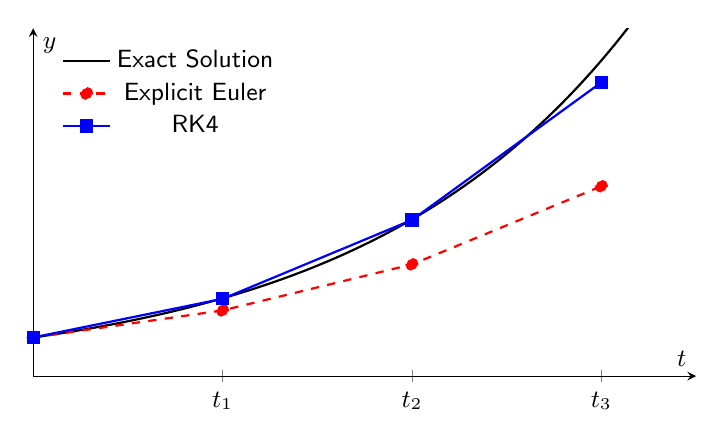
\begin{tikzpicture}[foundation]
        \begin{axis}[
            width=10cm, height=6cm,
            axis lines=middle,
            xlabel={$t$}, ylabel={$y$},
            xmin=0, xmax=3.5, ymin=0, ymax=4.5,
            xtick={0, 1, 2, 3}, xticklabels={$t_0$, $t_1$, $t_2$, $t_3$},
            ytick=\empty,
            legend pos=north west,
            legend style={draw=none, fill=none, font=\small\sffamily}
        ]
        % Exact curve
        \addplot[exact_curve, domain=0:3.2, samples=100] {0.5*exp(0.7*x)};
        \addlegendentry{Exact Solution}
        
        % Explicit Euler (linear steps)
        \addplot[approx_curve, mark=*] coordinates {(0, 0.5) (1, 0.85) (2, 1.445) (3, 2.456)};
        \addlegendentry{Explicit Euler}

        % RK4 (closer to exact)
        \addplot[symp_curve, mark=square*] coordinates {(0, 0.5) (1, 1.0) (2, 2.02) (3, 3.8)};
        \addlegendentry{RK4}
        \end{axis}
    \end{tikzpicture}
    \caption{Comparison of numerical integration methods. Explicit Euler unconditionally diverges for exponentially growing or stiff systems, while higher-order methods gracefully track the true continuous solution over short intervals.}
    \label{fig:integration_methods}
\end{figure}

It is crucial to emphasize that the mathematical validity of these classical explicit methods relies intrinsically on the global vector space structure. They mathematically construct the subsequent state by linearly scaling and directly adding derivative vectors ($h \bm{f}$) to the current base state ($\bm{y}_k$). As will be detailed later, if the simulated state manifold does not constitute a valid vector space (for example, if the state is constrained to represent a valid 3D rotation), naively adding Euclidean components will immediately force the state off the valid geometric manifold, leading to corrupted, non-physical states.

\subsection{Systems of ODEs and Higher-Order ODEs}
In the realm of classical physics, dynamic systems are predominantly described by higher-order differential equations. The most ubiquitous example is Newton's second law of motion, $\ddot{\bm{x}} = \bm{F}(t, \bm{x}, \dot{\bm{x}})/m$, which is inherently a second-order ODE. 
Fortunately, these higher-order constructs can be seamlessly handled using the exact same first-order integration techniques by systematically reducing them to a higher-dimensional system of first-order ODEs. By defining a composite phase-space state vector that explicitly includes the lower-order time derivatives, such as $\bm{y} = [\bm{x}^T, \dot{\bm{x}}^T]^T = [\bm{x}^T, \bm{v}^T]^T$, the generic second-order equation is elegantly transformed and rewritten as a coupled first-order system:
\begin{equation}
    \dot{\bm{y}} = \begin{bmatrix} \dot{\bm{x}} \\ \ddot{\bm{x}} \end{bmatrix} = \begin{bmatrix} \bm{v} \\ \frac{1}{m}\bm{F}(t, \bm{x}, \bm{v}) \end{bmatrix}
\end{equation}
This expanded state space representation is universally applicable, allowing any generic explicit or implicit ODE solver to be applied entirely transparently to physical systems of arbitrary dimension, complexity, and differential order.

\subsection{Symplectic Integrators and Error Bounds}
While standard explicit methods like RK4 offer highly accurate short-term local trajectories, they fundamentally fail to preserve the underlying geometric structure and symmetries of conservative Hamiltonian systems. In protracted physical simulations, such as orbital mechanics over thousands of years, this geometric failure manifests as a gradual, non-physical drift in the total mechanical energy—often leading to artificial orbital decay or expansion. 

Symplectic integrators represent a specialized class of numerical methods designed specifically to natively preserve the symplectic two-form of the Hamiltonian phase space (satisfying Liouville's theorem of phase space volume conservation). To mathematically understand their stability, we rely on \textit{Backward Error Analysis} (BEA). BEA reveals that instead of calculating an approximate, drifting solution to the exact continuous Hamiltonian $H$, a symplectic integrator computes the \textit{exact} continuous solution to a closely related "shadow" or modified Hamiltonian defined as $\tilde{H} = H + \mathcal{O}(h^p)$, where $p$ is the order of the method. 

In practical terms, this geometric preservation translates directly into the rigorous bounding of global energy errors. Instead of the total energy drifting monotonically over time (as occurs with standard explicit methods), the numerically computed energy of a symplectic integrator oscillates tightly around the true, exact energy level. This oscillation is strictly bounded by an error of $\mathcal{O}(h^p)$ for exponentially long times ($\mathcal{O}(e^{c/h})$), ensuring unparalleled long-term stability and physical fidelity.
Two notable, highly efficient symplectic methods include:
\begin{itemize}
    \item \textbf{Leapfrog Integration:} A second-order accurate method that evaluates positional and velocity data at interleaved, staggered time steps. It sequentially updates velocities at half-steps ($t_{k+1/2}$) and positions at integer steps ($t_{k+1}$). This alternating update scheme intrinsically provides excellent long-term energy stability while remaining computationally inexpensive.
    \item \textbf{Velocity Verlet:} A mathematically equivalent variation of the Leapfrog method that evaluates both positions and velocities at synchronized integer time steps. This formulation minimizes memory overhead and simplifies the integration with position-dependent forces, making it the de facto standard in molecular dynamics and complex rigid body physics engines.
\end{itemize}

\begin{figure}[htbp]
    \centering
    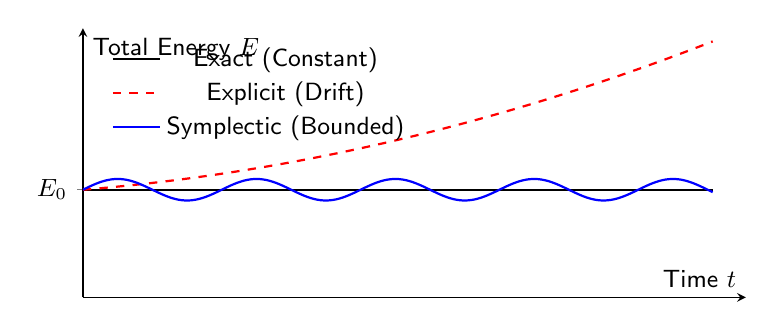
\begin{tikzpicture}[foundation]
        \begin{axis}[
            width=10cm, height=5cm,
            axis lines=middle,
            xlabel={Time $t$}, ylabel={Total Energy $E$},
            xmin=0, xmax=10, ymin=0, ymax=2.5,
            xtick=\empty, ytick={1}, yticklabels={$E_0$},
            legend pos=north west,
            legend style={draw=none, fill=none, font=\small\sffamily}
        ]
        % Exact energy
        \addplot[exact_curve, domain=0:9.5] {1};
        \addlegendentry{Exact (Constant)}
        
        % Explicit drift
        \addplot[approx_curve, domain=0:9.5, samples=100] {1 + 0.05*x + 0.01*x^2};
        \addlegendentry{Explicit (Drift)}
        
        % Symplectic oscillation
        \addplot[symp_curve, domain=0:9.5, samples=200] {1 + 0.1*sin(deg(3*x))};
        \addlegendentry{Symplectic (Bounded)}
        \end{axis}
    \end{tikzpicture}
    \caption{Energy conservation in conservative systems. Symplectic methods exhibit strictly bounded oscillations tightly around the exact initial energy, elegantly avoiding the secular, non-physical drift characteristic of standard explicit methods over long durations.}
    \label{fig:symplectic_energy}
\end{figure}

\section{Rigid Body Dynamics}
Having established a robust framework of numerical techniques required to simulate generalized differential equations, we now turn our focus to the specific physical laws governing rigid body dynamics. A rigid body is a theoretical idealization of a solid macroscopic object in which the spatial distance between any two internal constituent points remains perfectly constant, regardless of the magnitude or direction of external forces and torques applied to it.

\subsection{Translational Dynamics}
The translational motion of a rigid body, ignoring its orientation, is mathematically identical to that of an idealized point mass concentrated entirely at the body's geometric center of mass.
\begin{itemize}
    \item \textbf{Linear Momentum:} Formally defined as $\bm{p} = m \bm{v}$, where $m$ represents the total scalar mass of the rigid body and $\bm{v}$ denotes the instantaneous velocity vector of its center of mass relative to an inertial reference frame.
    \item \textbf{Newton's Second Law:} The fundamental principle stating that the time derivative of linear momentum is directly proportional to, and strictly equals, the vector sum of all external forces applied to the body: $\dot{\bm{p}} = \bm{F}_{\text{ext}}$. In the absence of net external forces, linear momentum is strictly conserved.
    \item \textbf{Energy:} The total mechanical energy $E$ of a conservative system is the sum of its kinetic and potential energies. The translational component of the kinetic energy is directly proportional to the square of the velocity magnitude: $K_{\text{trans}} = \frac{1}{2} m \|\bm{v}\|^2$.
\end{itemize}

\subsection{Rotational Dynamics}
The rotational behavior of a rigid body introduces complex angular counterparts to the translational equations, heavily dependent on the object's mass distribution:
\begin{itemize}
    \item \textbf{Angular Velocity ($\bm{\omega}$):} A 3D pseudovector (or axial vector) whose spatial direction dictates the instantaneous axis of rotation, and whose magnitude determines the rate of angular rotation in radians per second.
    \item \textbf{Center of Mass:} The unique internal equilibrium point where the weighted relative position vectors of the body's distributed mass sum precisely to zero. All unconstrained rotations naturally occur around this point.
    \item \textbf{Inertia Tensor ($\bm{I}$):} The intricate rotational equivalent of scalar mass. It is formulated as a $3 \times 3$ symmetric, positive-definite matrix that encapsulates exactly how the rigid body's mass is spatially distributed relative to the center of mass. The principal axes of this tensor define the natural axes of stable and unstable rotation.
    \item \textbf{Angular Momentum ($\bm{L}$):} The rotational analog to linear momentum, defined mathematically as the matrix-vector product $\bm{L} = \bm{I} \bm{\omega}$. The universally fundamental principle of conservation of angular momentum dictates that $\bm{L}$ remains absolutely constant over time if no net external torque acts upon the system.
    \item \textbf{Torque ($\bm{\tau}$):} The rotational equivalent of a linear force, representing a twisting force that causes a change in angular momentum over time, governed by Euler's rotational equation: $\dot{\bm{L}} = \bm{\tau}_{\text{ext}}$. Expanded in the body frame, this yields the non-linear Euler equations $\bm{I}\dot{\bm{\omega}} + \bm{\omega} \times (\bm{I}\bm{\omega}) = \bm{\tau}_{\text{ext}}$.
    \item \textbf{Total Kinetic Energy:} The complete kinetic energy of an unconstrained rigid body is the scalar sum of its independent translational and rotational kinetic energies: $K_{\text{total}} = \frac{1}{2} m \|\bm{v}\|^2 + \frac{1}{2} \bm{\omega}^T \bm{I} \bm{\omega}$.
\end{itemize}

\begin{figure}[htbp]
    \centering
    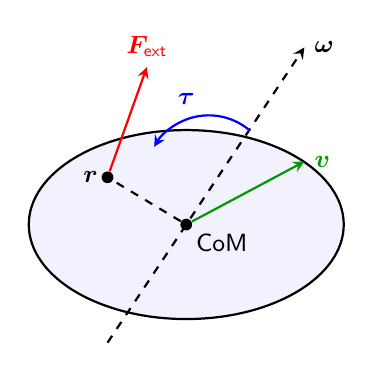
\begin{tikzpicture}[foundation]
        % Rigid body shape
        \draw[thick, fill=blue!5] (0,0) ellipse (2cm and 1.2cm);
        
        % Center of mass
        \node[particle] (com) at (0,0) {};
        \node[below right] at (com) {CoM};
        
        % Translational velocity
        \draw[velocity] (com) -- (1.5, 0.8) node[right] {$\bm{v}$};
        
        % Application point
        \node[particle] (p) at (-1, 0.6) {};
        \node[left] at (p) {$\bm{r}$};
        \draw[dashed, thick] (com) -- (p);
        
        % Force
        \draw[force] (p) -- (-0.5, 2) node[above] {$\bm{F}_{\text{ext}}$};
        
        % Rotation axis
        \draw[axis, dashed] (-1, -1.5) -- (1.5, 2.25) node[right] {$\bm{\omega}$};
        
        % Rotation arrow
        \draw[vector, ->] (0.8, 1.2) arc [start angle=50, end angle=150, radius=0.8cm];
        \node[blue] at (0, 1.6) {$\bm{\tau}$};
    \end{tikzpicture}
    \caption{Kinematics and dynamics of a rigid body. An external force $\bm{F}_{\text{ext}}$ applied at relative position $\bm{r}$ induces both a linear acceleration of the Center of Mass (CoM) and a torque $\bm{\tau}$ modifying the angular velocity $\bm{\omega}$.}
    \label{fig:rigid_body}
\end{figure}

\subsection{Inertia Tensor Computation}
The inertia tensor $\bm{I}$ of a continuous rigid body is a symmetric $3 \times 3$ matrix that quantitatively describes its mass distribution and determines the torque required for a desired angular acceleration about a given rotational axis. For a continuous body with mass density $\rho(\bm{r})$ distributed over a volume $V$, the inertia tensor evaluated at the origin is rigorously defined by the volume integral:
\begin{equation}
    \bm{I} = \iiint_V \rho(\bm{r}) \left( \|\bm{r}\|^2 \bm{1}_{3\times3} - \bm{r}\bm{r}^T \right) dV
\end{equation}
where $\bm{r} = [x, y, z]^T$ is the position vector of the infinitesimal mass element $dm = \rho(\bm{r}) dV$ relative to the origin, and $\bm{1}_{3\times3}$ is the identity matrix. Expanding the matrix components yields the diagonal \textit{moments of inertia} (e.g., $I_{xx} = \iiint \rho (y^2 + z^2) dV$) and the off-diagonal \textit{products of inertia} (e.g., $I_{xy} = -\iiint \rho xy \, dV$). 

In practical physics engines, bodies are often composed of primitive shapes (spheres, boxes, cylinders) or convex polyhedra. For these shapes, analytical solutions or discrete surface integrals exist to compute the local inertia tensor exactly around their respective centers of mass. When aggregating multiple shapes into a single composite rigid body, or when the rotation axis is shifted away from the center of mass, we employ the \textbf{Parallel Axis Theorem} (Steiner's theorem). For a body of mass $m$ and a center of mass inertia tensor $\bm{I}_c$, the translated inertia tensor $\bm{I}'$ relative to a new parallel coordinate frame displaced by a vector $\bm{d}$ is given by:
\begin{equation}
    \bm{I}' = \bm{I}_c + m \left( \|\bm{d}\|^2 \bm{1}_{3\times3} - \bm{d}\bm{d}^T \right)
\end{equation}
This algebraic transformation avoids computationally expensive numerical integration by shifting previously known, exact primitive tensors to a common shared coordinate frame.

\section{Rotational Representations and Lie Groups}

\subsection{Introduction to Lie Groups}
To numerically integrate complex rotational dynamics accurately over time, we must first establish a mathematically robust representation for 3D spatial rotations. From an intuitive engineering and physics perspective, a Lie group acts as a continuous, smooth mathematical manifold—a curved topological space that, on a purely local level, resembles flat Euclidean space—but simultaneously possesses the rigid algebraic structure of a group, meaning elements can be continuously multiplied and smoothly inverted. 
When simulating unconstrained 3D rotations, we predominantly focus on two specific, interrelated Lie groups:
\begin{itemize}
    \item \textbf{Special Orthogonal Group $\text{SO}(3)$:} The classical matrix group encompassing all $3 \times 3$ orthogonal matrices that strictly satisfy the condition $\bm{R}^T\bm{R} = \bm{I}$ with a positive determinant of $\det(\bm{R}) = +1$. This directly represents length-preserving and handedness-preserving rigid rotations.
    \item \textbf{Unit Quaternions $\text{Sp}(1)$ or $\text{SU}(2)$:} A specific mathematical subset of 4D hypercomplex numbers forming a closed unit hypersphere (denoted $S^3$) in 4D space. Represented as $\bm{q} = [q_w, q_x, q_y, q_z]$, unit quaternions offer an extremely compact, computationally efficient, and intrinsically singularity-free representation. Crucially, they completely avoid the "Gimbal lock" phenomenon that plagues traditional Euler angle representations.
\end{itemize}

\subsection{Lie Algebras and the Hat Operator}
The tangent vector space evaluated precisely at the identity element of any Lie group forms its corresponding Lie algebra. This algebraic structure elegantly represents the space of all possible infinitesimal rotational transformations (i.e., rotational velocities). For the specific case of $\text{SO}(3)$, its Lie algebra, denoted as $\mathfrak{so}(3)$, corresponds to the mathematical space of all $3 \times 3$ skew-symmetric matrices. The instantaneous angular velocity pseudovector $\bm{\omega}$ inherently and exclusively resides within this specific algebra.
To rigorously bridge the gap between 3D vectors and matrices, we define the "hat" operator $\widehat{(\cdot)}$ to uniquely map a standard 3D pseudovector $\bm{\omega} \in \mathbb{R}^3$ directly to its exact matrix representation within $\mathfrak{so}(3)$:
\begin{equation}
    \widehat{\bm{\omega}} = \begin{bmatrix} 0 & -\omega_z & \omega_y \\ \omega_z & 0 & -\omega_x \\ -\omega_y & \omega_x & 0 \end{bmatrix}
\end{equation}
When mathematically applying this hat-transformed matrix to another generic spatial vector, it perfectly retro-projects the operation, acting identically to a standard vector cross product: $\widehat{\bm{\omega}} \bm{v} = \bm{\omega} \times \bm{v}$.
For unit quaternions, the derivative mapping from the physical angular velocity $\bm{\omega}$ to the mathematical rate of change of the quaternion itself, $\dot{\bm{q}}$, requires a specialized matrix hat operator acting dynamically on the 4D state space. This mapping typically takes the compact algebraic form $\dot{\bm{q}} = \frac{1}{2} \widehat{\bm{\omega}}_q \bm{q}$, where the operator $\widehat{\bm{\omega}}_q$ is systematically constructed using the 3D spatial components of $\bm{\omega}$.

\subsection{Numerical Integration on Manifolds}
Given these non-Euclidean geometries, it becomes fundamentally apparent that numerical integration algorithms designed purely for flat vector spaces require the intermediary use of Lie algebras to function correctly. If one were to naively attempt to use Explicit Euler to directly update a rotation matrix by adding a scaled linear derivative ($\bm{R}_{k+1} = \bm{R}_k + h \dot{\bm{R}}$), the resulting updated matrix $\bm{R}_{k+1}$ would definitively no longer be strictly orthogonal. By simply adding matrices, the state violently leaves the highly constrained $\text{SO}(3)$ manifold. 

To circumvent this, we must formally map the current rotational state into the locally flat Lie algebra using the hat operator, perform the linear numerical integration safely within the valid, unconstrained vector space of the algebra, and ultimately project the resultant state back onto the curved Lie group manifold. This final projection is flawlessly executed utilizing the exact matrix exponential map, denoted $\exp: \mathfrak{so}(3) \to \text{SO}(3)$. For a rotation vector $\Delta\bm{\theta} = \bm{\omega} h$ with magnitude $\theta = \|\Delta\bm{\theta}\|$ and normalized axis $\bm{u} = \Delta\bm{\theta} / \theta$, the closed-form evaluation of this matrix exponential yields the renowned Rodrigues' rotation formula:
\begin{equation}
    \exp(\widehat{\Delta\bm{\theta}}) = \bm{1}_{3\times3} + \sin(\theta) \widehat{\bm{u}} + (1 - \cos(\theta)) \widehat{\bm{u}}^2
\end{equation}
The discrete update for the rotation matrix then becomes a multiplicative Lie group operation: $\bm{R}_{k+1} = \bm{R}_k \exp(\widehat{\bm{\omega}} h)$. 

An analogous, highly efficient exponential map exists for unit quaternions mapping from $\mathfrak{su}(2) \to \text{SU}(2)$:
\begin{equation}
    \exp_{q}(\Delta\bm{\theta}) = \left[ \cos\left(\frac{\theta}{2}\right), \bm{u} \sin\left(\frac{\theta}{2}\right) \right]^T
\end{equation}
where the update is performed using quaternion multiplication: $\bm{q}_{k+1} = \bm{q}_k \otimes \exp_{q}(\bm{\omega} h)$. This comprehensive methodology, broadly known as Lie Group Integration, geometrically guarantees the state remains exactly on the valid mathematical manifold at all times without requiring arbitrary, physically unmotivated artificial re-normalization steps.

\begin{figure}[htbp]
    \centering
    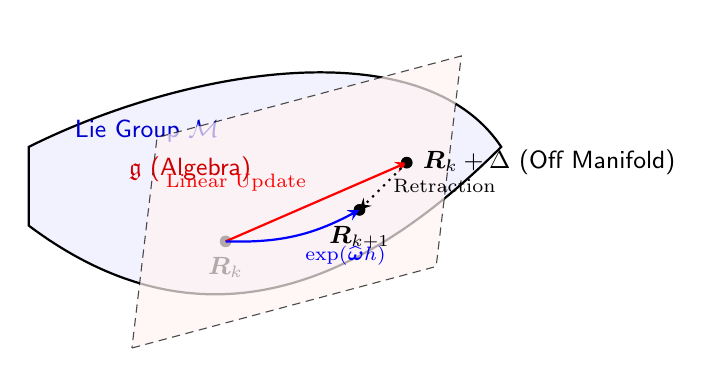
\begin{tikzpicture}[foundation]
        % Manifold surface
        \draw[thick, fill=blue!5] (0,1) .. controls (2,-0.5) and (4,0) .. (6,2) .. controls (5,3.5) and (2,3) .. (0,2) -- cycle;
        \node[blue!80!black] at (1.5, 2.2) {Lie Group $\mathcal{M}$};
        
        % Point R_k
        \coordinate (Rk) at (2.5, 0.8);
        \node[particle, label=below:$\bm{R}_k$] at (Rk) {};
        
        % Tangent plane (Lie Algebra)
        \begin{scope}[shift={(Rk)}, rotate=15]
            \draw[fill=red!5, opacity=0.7, densely dashed] (-1.5,-1) -- (2.5,-1) -- (3.5,1.5) -- (-0.5,1.5) -- cycle;
            \node[red!80!black] at (-0.2, 1) {$\mathfrak{g}$ (Algebra)};
        \end{scope}
        
        % Explicit step (in tangent plane)
        \coordinate (Explicit) at (4.8, 1.8);
        \node[particle, label=right:{$\bm{R}_k + \Delta$ (Off Manifold)}] at (Explicit) {};
        \draw[arrow, red, thick] (Rk) -- (Explicit) node[midway, above left, font=\scriptsize] {Linear Update};
        
        % Projected point R_{k+1}
        \coordinate (Rk1) at (4.2, 1.2);
        \node[particle, label=below:$\bm{R}_{k+1}$] at (Rk1) {};
        
        % Curve on manifold
        \draw[arrow, blue, thick] (Rk) to[bend right=15] node[midway, below right, font=\scriptsize] {$\exp(\widehat{\bm{\omega}} h)$} (Rk1);
        
        % Projection line
        \draw[arrow, black, dotted] (Explicit) -- (Rk1) node[midway, right, font=\scriptsize] {Retraction};

    \end{tikzpicture}
    \caption{Lie Group Integration. Standard linear updates push the state off the curved manifold. Lie group methods utilize the local Lie algebra and the exponential map to seamlessly advance the state along the true geometric surface.}
    \label{fig:lie_group_integration}
\end{figure}

\section{Implicit Integration Methods}

\subsection{Root-Finding and Newton-Raphson}
While explicit integration methods are computationally straightforward and exceptionally easy to implement, they suffer from a fatal flaw when applied to "stiff" differential equations—systems where physical components naturally evolve on vastly disparate, competing timescales. For stiff systems, explicit methods require prohibitively infinitesimal time steps to avoid catastrophic numerical explosion. Implicit methods gracefully resolve this instability by radically changing the evaluation point: they evaluate the requisite vector field at the yet-unknown future time step $t_{k+1}$.
Mathematically, this necessitates formulating and solving a complex nonlinear algebraic equation of the form $\bm{F}(\bm{y}_{k+1}) = \bm{0}$ at every single integration step.
The Newton-Raphson algorithm is a dominant, universally applied iterative root-finding technique tailored for solving such nonlinear systems. It utilizes local derivative information to iteratively converge on the true solution:
\begin{equation}
    \bm{y}^{(i+1)}_{k+1} = \bm{y}^{(i)}_{k+1} - \left[ \nabla \bm{F}\left(\bm{y}^{(i)}_{k+1}\right) \right]^{-1} \bm{F}\left(\bm{y}^{(i)}_{k+1}\right)
\end{equation}
where $\nabla \bm{F}$ denotes the exact, analytically derived Jacobian matrix of the system. 

For complex physical simulations where the analytical Jacobian is either mathematically intractable to derive or overwhelmingly computationally expensive to continually evaluate and invert, quasi-Newton secant approximations—such as the renowned Broyden method—can be seamlessly substituted. Broyden's method iteratively and efficiently approximates the Jacobian $\bm{B} \approx \nabla \bm{F}$ (or its direct inverse) on-the-fly using only the function evaluations from consecutive steps. Defining the state difference $\Delta \bm{y} = \bm{y}^{(i+1)} - \bm{y}^{(i)}$ and the function difference $\Delta \bm{F} = \bm{F}(\bm{y}^{(i+1)}) - \bm{F}(\bm{y}^{(i)})$, the secant update for the approximate Jacobian is:
\begin{equation}
    \bm{B}_{i+1} = \bm{B}_i + \frac{\Delta \bm{F} - \bm{B}_i \Delta \bm{y}}{\|\Delta \bm{y}\|^2} \Delta \bm{y}^T
\end{equation}
This approach sacrifices exact quadratic convergence for superlinear convergence, dramatically drastically reducing the per-iteration computational cost by eliminating the need to re-evaluate the full analytical Jacobian matrix.

\begin{figure}[htbp]
    \centering
    \begin{tikzpicture}[foundation]
        \begin{axis}[
            width=10cm, height=6cm,
            axis x line=middle, axis y line=left,
            xlabel={$y$}, ylabel={$F(y)$},
            xmin=0, xmax=3.5, ymin=-1.5, ymax=4,
            xtick={1.414, 1.833, 3}, xticklabels={$y^*$, $y^{(i+1)}$, $y^{(i)}$},
            ytick=\empty,
            every axis x label/.style={at={(ticklabel* cs:1)},anchor=west},
            every axis y label/.style={at={(ticklabel* cs:1)},anchor=south}
        ]
        % Function F(y) = 0.5*x^2 - 1
        \addplot[exact_curve, domain=0.5:3.2, samples=100] {0.5*x^2 - 1};
        \node[right] at (axis cs:3.2, 4) {$F(y)$};
        
        % Root
        \node[particle] at (axis cs:1.414, 0) {};
        
        % Point at y(i)
        \draw[dashed, gray] (axis cs:3, 0) -- (axis cs:3, 3.5);
        \node[particle] (Pi) at (axis cs:3, 3.5) {};
        
        % Tangent from y(i)
        \addplot[approx_curve, domain=1.5:3.2] {3*x - 5.5};
        
        % Point at y(i+1)
        \draw[dashed, gray] (axis cs:1.833, 0) -- (axis cs:1.833, 0.68);
        \node[particle] (Pip1) at (axis cs:1.833, 0.68) {};
        
        % Tangent from y(i+1)
        \addplot[approx_curve, domain=1.2:2.2] {1.833*x - 2.68};

        \end{axis}
    \end{tikzpicture}
    \caption{The Newton-Raphson method for root-finding. By iteratively evaluating the function and its local derivative (tangent line, dashed red), the sequence of estimates $y^{(i)}$ rapidly converges towards the true root $y^*$.}
    \label{fig:newton_raphson}
\end{figure}

\subsection{Implicit Integration}
Equipped with powerful numerical root-finding capabilities, we can successfully deploy advanced, highly robust implicit integrators. The Implicit Midpoint Rule serves as an exemplary gold standard for such methods:
\begin{equation}
    \bm{y}_{k+1} = \bm{y}_k + h \bm{f}\left(t_k + \frac{h}{2}, \frac{\bm{y}_k + \bm{y}_{k+1}}{2}\right)
\end{equation}
Rather than evaluating at the boundaries, this elegant formulation evaluates the state derivative precisely at the temporal midpoint of the integration step, utilizing the arithmetic average of the known current state and the unknown future state. Mathematically, the Implicit Midpoint Rule is unconditionally A-stable for linear systems (meaning integration will not mathematically explode regardless of step size), is formally second-order accurate in time, and, perhaps most critically for physics engines, belongs to the elite class of symplectic integrators. This rare trifecta—combining unconditional stability with rigorous geometric energy preservation—makes it an exceptionally favorable and deeply reliable choice for stiff, long-duration physical simulations where both unwavering numerical stability and strict adherence to conservation laws are paramount.

\section{Coupled Particle and Rigid Body Integration}

To construct a robust, mathematically rigorous integration scheme for a mutually coupled system of particles and a rigid body, we must unify two powerful geometric integrators: Velocity Verlet (VV) for the Euclidean particle space $\mathbb{R}^{3N}$ and the Implicit Midpoint Rule (IMR) on a Lie Group for the rigid body manifold $\mathbb{R}^3 \times \text{SO}(3)$. Both integrators share two fundamental properties: they are symmetric (time-reversible) and second-order accurate $\mathcal{O}(h^2)$. However, Velocity Verlet is explicit in its position updates, whereas IMR is fully implicit. By interleaving the explicit kicks of the particles with the implicit Lie group solve of the rigid body, we create a Partitioned Implicit-Explicit (IMEX) scheme. This synchronizes all force evaluations exactly at the time midpoint $t_{n+1/2}$, guaranteeing symplectic-like structure preservation while restricting the expensive implicit root-finding purely to the $6 \times 6$ rigid body space. Here is the in-depth mathematical derivation of the continuous formulation, the coupled discrete algorithm, the analytical $\text{SO}(3)$ Jacobian, and the proof of reversibility.

\subsection{Configuration Manifolds and Continuous Dynamics}
Let the system consist of $N$ particles and a single rigid body. We decouple the rigid body's Euclidean translation from its non-Euclidean rotation to avoid the translation-rotation velocity coupling inherent to the $\text{SE}(3)$ exponential map.

\textbf{Particle System ($\mathbb{R}^{3N}$):}\\
For particles with positions $\mathbf{q} \in \mathbb{R}^{3N}$, velocities $\mathbf{v} \in \mathbb{R}^{3N}$, and diagonal mass matrix $\mathbf{M}_p$:
\begin{equation}
    \dot{\mathbf{q}} = \mathbf{v}, \quad \mathbf{M}_p \dot{\mathbf{v}} = \mathbf{F}_p(\mathbf{q}, \mathbf{x}, \mathbf{R})
\end{equation}

\textbf{Rigid Body System ($\mathbb{R}^3 \times \text{SO}(3)$):}\\
Let $\mathbf{x} \in \mathbb{R}^3$ be the center of mass, $\mathbf{v}_{rb} \in \mathbb{R}^3$ the world-frame linear velocity, and $M$ the mass. Let $\mathbf{R} \in \text{SO}(3)$ be the orientation, $\boldsymbol{\omega} \in \mathbb{R}^3$ the body-frame angular velocity, and $\mathbf{J} \in \mathbb{R}^{3\times3}$ the constant body-frame inertia tensor.
\begin{align}
    \dot{\mathbf{x}} &= \mathbf{v}_{rb}, \quad M \dot{\mathbf{v}}_{rb} = \mathbf{F}_{rb}(\mathbf{q}, \mathbf{x}, \mathbf{R}) \\
    \dot{\mathbf{R}} &= \mathbf{R} \widehat{\boldsymbol{\omega}}, \quad \mathbf{J}\dot{\boldsymbol{\omega}} + \boldsymbol{\omega} \times \mathbf{J}\boldsymbol{\omega} = \boldsymbol{\tau}_{body}(\mathbf{q}, \mathbf{x}, \mathbf{R})
\end{align}
(Note: $\widehat{\boldsymbol{\omega}} \in \mathfrak{so}(3)$ is the skew-symmetric matrix such that $\widehat{\boldsymbol{\omega}}\mathbf{a} = \boldsymbol{\omega} \times \mathbf{a}$.)

\subsection{The Staggered IMEX Integration Loop}
To advance the state from $t_n$ to $t_{n+1}$ over interval $h$, we split the Velocity Verlet into two halves and nest the Implicit Midpoint Rule exactly between them.

\textbf{Phase 1: Particle Explicit Velocity Half-Kick}\\
Evaluate forces at the starting configuration $t_n$ and advance particle velocities by a half-step:
\begin{equation}
    \mathbf{v}_{n+1/2} = \mathbf{v}_n + \frac{h}{2} \mathbf{M}_p^{-1} \mathbf{F}_p(\mathbf{q}_n, \mathbf{x}_n, \mathbf{R}_n)
\end{equation}

\textbf{Phase 2: Particle Drift to Midpoint (Synchronization)}\\
Advance the particle positions exactly to the integration midpoint $t_{n+1/2}$:
\begin{equation}
    \mathbf{q}_{mid} = \mathbf{q}_n + \frac{h}{2} \mathbf{v}_{n+1/2}
\end{equation}
Crucially, $\mathbf{q}_{mid}$ is now explicitly known. We freeze it to solve the implicit rigid body step.

\textbf{Phase 3: Lie Group Implicit Solve (Rigid Body)}\\
We define the rigid body midpoint velocities as the unknown variables $\mathbf{v}_{mid}$ and $\boldsymbol{\omega}_{mid}$. The midpoint configuration is evaluated using linear translation and the $\text{SO}(3)$ Lie Group exponential map (Rodrigues' formula):
\begin{equation}
    \mathbf{x}_{mid} = \mathbf{x}_n + \frac{h}{2} \mathbf{v}_{mid}, \quad \mathbf{R}_{mid} = \mathbf{R}_n \exp\left( \frac{h}{2} \widehat{\boldsymbol{\omega}}_{mid} \right)
\end{equation}
We substitute the discrete velocities $\dot{\mathbf{v}}_{rb} \approx \frac{2}{h}(\mathbf{v}_{mid} - \mathbf{v}_{rb, n})$ into the Newton-Euler equations evaluated at $t_{n+1/2}$. This yields a $6 \times 6$ non-linear root-finding problem $\mathbf{G}(\mathbf{v}_{mid}, \boldsymbol{\omega}_{mid}) = \mathbf{0}$:
\begin{align}
    \mathbf{G}_v &= \frac{2M}{h} (\mathbf{v}_{mid} - \mathbf{v}_{rb, n}) - \mathbf{F}_{rb}(\mathbf{q}_{mid}, \mathbf{x}_{mid}, \mathbf{R}_{mid}) = \mathbf{0} \\
    \mathbf{G}_\omega &= \frac{2}{h} \mathbf{J} (\boldsymbol{\omega}_{mid} - \boldsymbol{\omega}_n) + \boldsymbol{\omega}_{mid} \times \mathbf{J} \boldsymbol{\omega}_{mid} - \boldsymbol{\tau}_{body}(\mathbf{q}_{mid}, \mathbf{x}_{mid}, \mathbf{R}_{mid}) = \mathbf{0}
\end{align}
(We solve this iteratively via Newton-Raphson. The exact geometric Jacobian is derived in Section 1.5.4).

\textbf{Phase 4: Rigid Body Full State Update}\\
Once Phase 3 converges to the exact roots $\mathbf{v}_{mid}^*$ and $\boldsymbol{\omega}_{mid}^*$, we definitively finalize the rigid body state at $t_{n+1}$:
\begin{align}
    \mathbf{x}_{n+1} &= \mathbf{x}_n + h \mathbf{v}_{mid}^* \\
    \mathbf{R}_{n+1} &= \mathbf{R}_n \exp\left( h \widehat{\boldsymbol{\omega}}_{mid}^* \right) \\
    \mathbf{v}_{rb, n+1} &= 2\mathbf{v}_{mid}^* - \mathbf{v}_{rb, n} \\
    \boldsymbol{\omega}_{n+1} &= 2\boldsymbol{\omega}_{mid}^* - \boldsymbol{\omega}_n
\end{align}

\textbf{Phase 5: Particle Second Drift and Kick}\\
Advance the particles to $t_{n+1}$ and complete the Velocity Verlet loop:
\begin{align}
    \mathbf{q}_{n+1} &= \mathbf{q}_{mid} + \frac{h}{2} \mathbf{v}_{n+1/2} \\
    \mathbf{v}_{n+1} &= \mathbf{v}_{n+1/2} + \frac{h}{2} \mathbf{M}_p^{-1} \mathbf{F}_p(\mathbf{q}_{n+1}, \mathbf{x}_{n+1}, \mathbf{R}_{n+1})
\end{align}

\begin{figure}[htbp]
    \centering
    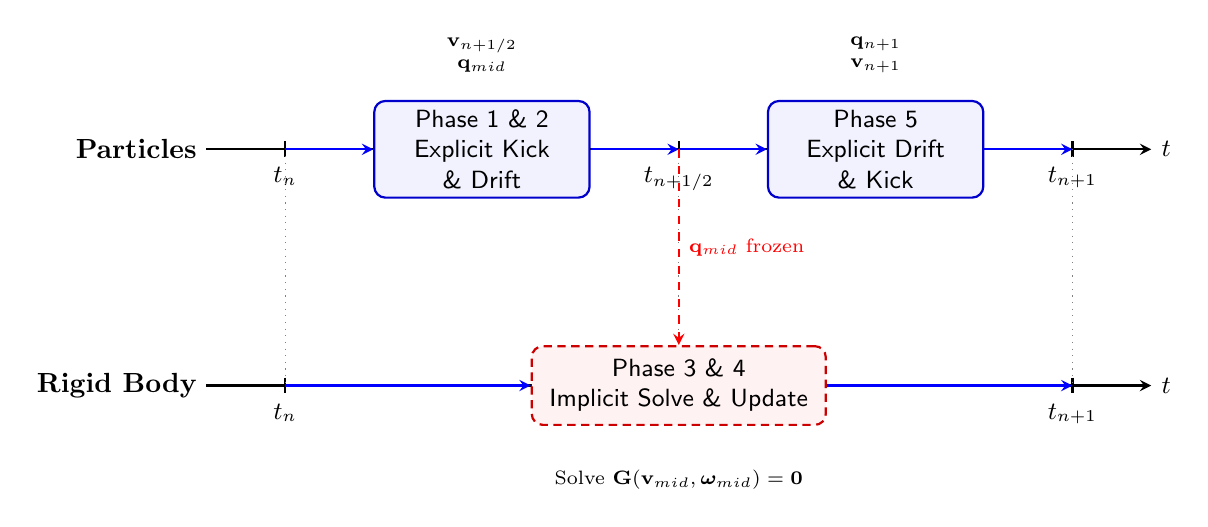
\begin{tikzpicture}[foundation]
        % Timeline axes
        \draw[axis] (0, 0) -- (12, 0) node[right] {$t$};
        \draw[axis] (0, -3) -- (12, -3) node[right] {$t$};
        
        \node[left, font=\bfseries] at (0, 0) {Particles};
        \node[left, font=\bfseries] at (0, -3) {Rigid Body};
        
        % Time ticks
        \foreach \x/\l in {1/$t_n$, 6/$t_{n+1/2}$, 11/$t_{n+1}$} {
            \draw[thick] (\x, 0.1) -- (\x, -0.1) node[below] {\l};
            \draw[thick] (\x, -2.9) -- (\x, -3.1) node[below] {\l};
            \draw[dotted, gray] (\x, 0) -- (\x, -3);
        }
        
        % Nodes
        \node[block, text width=2.5cm] (kick1) at (3.5, 0) {Phase 1 \& 2\\Explicit Kick \& Drift};
        \node[block, text width=2.5cm] (kick2) at (8.5, 0) {Phase 5\\Explicit Drift \& Kick};
        
        \node[implicit_block, text width=3.5cm] (implicit) at (6, -3) {Phase 3 \& 4\\Implicit Solve \& Update};
        
        % Arrows
        \draw[arrow, blue] (1, 0) -- (kick1);
        \draw[arrow, blue] (kick1) -- (6, 0);
        \draw[arrow, blue] (6, 0) -- (kick2);
        \draw[arrow, blue] (kick2) -- (11, 0);
        
        \draw[arrow, red, dashed, thick] (6, 0) -- (implicit) node[midway, right, font=\scriptsize] {$\mathbf{q}_{mid}$ frozen};
        \draw[arrow, blue] (1, -3) -- (implicit);
        \draw[arrow, blue] (implicit) -- (11, -3);
        
        \node[align=center, font=\scriptsize] at (3.5, 1.2) {$\mathbf{v}_{n+1/2}$\\$\mathbf{q}_{mid}$};
        \node[align=center, font=\scriptsize] at (8.5, 1.2) {$\mathbf{q}_{n+1}$\\$\mathbf{v}_{n+1}$};
        
        \node[align=center, font=\scriptsize] at (6, -4.2) {Solve $\mathbf{G}(\mathbf{v}_{mid}, \boldsymbol{\omega}_{mid}) = \mathbf{0}$};
        
    \end{tikzpicture}
    \caption{Partitioned Implicit-Explicit (IMEX) timeline. The particle system is explicitly stepped using a split Velocity Verlet scheme, which perfectly synchronizes the configuration exactly at the midpoint $t_{n+1/2}$. This intermediate state is locked to evaluate the computationally expensive implicit rigid body Newton-Euler solver before advancing both systems to $t_{n+1}$.}
    \label{fig:imex_loop}
\end{figure}

\subsection{Proof of Exact Time-Reversibility}
A numerical integrator is strictly time-reversible if starting from state $S_{n+1}$, negating the velocities, and taking a step of size $-h$ perfectly yields the original state $S_n$. This property bounds energy drift indefinitely.

Let's trace the algorithm backwards from $t_{n+1}$ with step $-h$:
\begin{itemize}
    \item \textbf{Reverse Phase 1:} $\mathbf{v}_{mid}^* = -\mathbf{v}_{n+1} + \frac{-h}{2}\mathbf{M}_p^{-1} \mathbf{F}_p(t_{n+1})$. Based on forward Phase 5, this explicitly evaluates to $-\mathbf{v}_{n+1/2}$.
    \item \textbf{Reverse Phase 2:} $\mathbf{q}_{mid}^* = \mathbf{q}_{n+1} + \frac{-h}{2} (-\mathbf{v}_{n+1/2}) = \mathbf{q}_{n+1} - \frac{h}{2} \mathbf{v}_{n+1/2} = \mathbf{q}_{mid}$.
    \item \textbf{Reverse Phase 3:} Because $\mathbf{q}_{mid}$ is identical, the implicit rigid body solver experiences the exact same environment. If we evaluate the residual using guesses $-\mathbf{v}_{mid}$ and $-\boldsymbol{\omega}_{mid}$, the backward midpoint geometries evaluate to:
\begin{align}
    \mathbf{x}_{mid}^* &= \mathbf{x}_{n+1} + \frac{-h}{2}(-\mathbf{v}_{mid}) = \mathbf{x}_n + h\mathbf{v}_{mid} + \frac{h}{2}\mathbf{v}_{mid} = \mathbf{x}_{mid} \\
    \mathbf{R}_{mid}^* &= \mathbf{R}_{n+1} \exp\left( \frac{-h}{2} (-\widehat{\boldsymbol{\omega}}_{mid}) \right) = \mathbf{R}_n \exp(h\widehat{\boldsymbol{\omega}}_{mid}) \exp\left(-\frac{h}{2}\widehat{\boldsymbol{\omega}}_{mid}\right) = \mathbf{R}_{mid}
\end{align}
    Since the configurations perfectly match, the coupling forces are identical. The inertial derivative $\frac{2}{-h}(-\mathbf{v}_{mid} - (-\mathbf{v}_{rb, n+1}))$ algebraically simplifies to exactly $\frac{2}{h}(\mathbf{v}_{mid} - \mathbf{v}_{rb, n})$. Thus, $\mathbf{G}^* = \mathbf{G} = \mathbf{0}$, meaning the exact negative mid-velocities are recovered.
    \item \textbf{Reverse Phases 4 \& 5:} By symmetry, applying $-h$ with the converged roots perfectly recovers $\mathbf{x}_n, \mathbf{R}_n, \mathbf{v}_{rb, n}, \boldsymbol{\omega}_n$, and $\mathbf{v}_n$.
\end{itemize}

\subsection{In-Depth Analytical Jacobian on Lie Group \texorpdfstring{$\text{SO}(3)$}{SO(3)}}
To solve Phase 3 in 2-3 iterations, we need the exact $6 \times 6$ Newton-Raphson block Jacobian $\mathcal{J} = \frac{\partial (\mathbf{G}_v, \mathbf{G}_\omega)}{\partial (\mathbf{v}_{mid}, \boldsymbol{\omega}_{mid})}$.
Let the coupling force $\mathbf{F}_{world}$ apply at a constant body-frame attachment point $\mathbf{p}$. The body torque is $\boldsymbol{\tau}_{body} = \mathbf{p} \times (\mathbf{R}_{mid}^T \mathbf{F}_{world})$. Let $\mathbf{K} = \frac{\partial \mathbf{F}_{world}}{\partial \mathbf{x}_{world}}$ be the $3 \times 3$ translational stiffness matrix evaluated at the world point.

\textbf{A. Lie Group Variations}\\
If we perturb the midpoint angular velocity by $\delta \boldsymbol{\omega}_{mid}$, the right-trivialized tangent of the exponential map defines the variation in rotation $\delta \mathbf{R}_{mid}$:
\begin{equation}
    \delta \mathbf{R}_{mid} = \mathbf{R}_{mid} \widehat{\delta \boldsymbol{\phi}} \quad \text{where} \quad \delta \boldsymbol{\phi} = \frac{h}{2} \mathbf{J}_r\left(\frac{h}{2} \boldsymbol{\omega}_{mid}\right) \delta \boldsymbol{\omega}_{mid}
\end{equation}
Here, $\mathbf{J}_r(\boldsymbol{\theta})$ is the Right Jacobian of $\text{SO}(3)$:
\begin{equation}
    \mathbf{J}_r(\boldsymbol{\theta}) = \mathbf{I} - \frac{1 - \cos\|\boldsymbol{\theta}\|}{\|\boldsymbol{\theta}\|^2} \widehat{\boldsymbol{\theta}} + \frac{\|\boldsymbol{\theta}\| - \sin\|\boldsymbol{\theta}\|}{\|\boldsymbol{\theta}\|^3} \widehat{\boldsymbol{\theta}}^2
\end{equation}

\textbf{B. Force and Torque Derivatives}\\
By tracking the variations of $\mathbf{x}_{mid}$ and $\mathbf{R}_{mid}$ induced by $\delta \mathbf{v}_{mid}$ and $\delta \boldsymbol{\omega}_{mid}$, we find the variation of the attachment point, and subsequently $\delta \mathbf{F}_{world}$ and $\delta \boldsymbol{\tau}_{body}$. Applying the chain rule and the identity $\widehat{\mathbf{a}}\mathbf{b} = -\widehat{\mathbf{b}}\mathbf{a}$, we extract the four blocks of the analytic Jacobian:

\textbf{1. Translational Block ($3 \times 3$):}
\begin{equation}
    \frac{\partial \mathbf{G}_v}{\partial \mathbf{v}_{mid}} = \frac{2M}{h} \mathbf{I} - \frac{h}{2} \mathbf{K}
\end{equation}

\textbf{2. Translational-Rotational Coupling Block ($3 \times 3$):}
\begin{equation}
    \frac{\partial \mathbf{G}_v}{\partial \boldsymbol{\omega}_{mid}} = \frac{h}{2} \mathbf{K} \mathbf{R}_{mid} \widehat{\mathbf{p}} \mathbf{J}_r
\end{equation}

\textbf{3. Rotational-Translational Coupling Block ($3 \times 3$):}
\begin{equation}
    \frac{\partial \mathbf{G}_\omega}{\partial \mathbf{v}_{mid}} = -\frac{h}{2} \widehat{\mathbf{p}} \mathbf{R}_{mid}^T \mathbf{K}
\end{equation}

\textbf{4. Rotational Block ($3 \times 3$):}\\
The rotational block contains the derivative of the Coriolis term $\frac{\partial}{\partial \boldsymbol{\omega}} (\boldsymbol{\omega} \times \mathbf{J}\boldsymbol{\omega}) = \widehat{\boldsymbol{\omega}}\mathbf{J} - \widehat{\mathbf{J}\boldsymbol{\omega}}$, combined with the Lie-mapped geometric stiffness:
\begin{equation}
    \frac{\partial \mathbf{G}_\omega}{\partial \boldsymbol{\omega}_{mid}} = \frac{2}{h} \mathbf{J} + \widehat{\boldsymbol{\omega}}_{mid} \mathbf{J} - \widehat{\mathbf{J} \boldsymbol{\omega}_{mid}} - \frac{h}{2} \left[ \widehat{\mathbf{p}} \left( \mathbf{R}_{mid}^T \mathbf{F}_{world} \right)^\wedge - \widehat{\mathbf{p}} \mathbf{R}_{mid}^T \mathbf{K} \mathbf{R}_{mid} \widehat{\mathbf{p}} \right] \mathbf{J}_r
\end{equation}
(Where $\mathbf{J}_r \equiv \mathbf{J}_r(\frac{h}{2}\boldsymbol{\omega}_{mid})$). If multiple particles attach to the rigid body, you simply sum the stiffness contributions $\mathbf{K}_j$ and points $\mathbf{p}_j$ across these blocks.

\textbf{Summary}\\
By locking the explicit midpoint configuration $\mathbf{q}_{mid}$ during the implicit rigid body step, this IMEX formulation circumvents a massive $(3N+6) \times (3N+6)$ coupled Jacobian inversion. Instead, you only ever invert a dense $6 \times 6$ matrix, yielding a highly scalable algorithm that perfectly maintains $\mathcal{O}(h^2)$ precision, temporal symmetry, and exact adherence to the $\text{SO}(3)$ manifold.

\printbibliography[
heading=bibintoc,
]

\end{document}